\documentclass{article}

\usepackage{color}
\usepackage[top=1in,bottom=1in,left=1.2in,right=1.2in]{geometry}
\usepackage{hyperref}
\usepackage[small]{titlesec}
\usepackage{booktabs}
\usepackage{colm2024_conference}
\usepackage{graphicx}
\usepackage[dvipsnames]{xcolor}
\usepackage{rotating}
\usepackage{pdflscape}
\usepackage{amsmath}

\newcommand{\todo}[1]{\textcolor{red}{\textbf{TODO:} #1}}

% Commenting
\newcommand{\eat}[1]{\ignorespaces}
%% Comment this line and uncomment the next to hide all comments
\newcommand{\xxcomment}[4]{\textcolor{#1}{[$^{\textsc{#2}}_{\textsc{#3}}$ #4]}}
%\newcommand{\xxcomment}[4]{\eat{#1}}
\newcommand{\ya}[1]{\xxcomment{red}{Y}{A}{#1}}
\newcommand{\ta}[1]{\xxcomment{blue}{T}{A}{#1}}


\title{CSE 5525: Assignment 3}

\author{Abhiram Rustagi}


\date{\today}


\colmfinalcopy
\begin{document}
\maketitle


\section{Data Statistics and Processing (8pt)}
\paragraph{Instructions:} Use \autoref{tab:data_stats_before} and \autoref{tab:data_stats_after} to describe the data statistics before and after any pre-processing respectively. 
Use the T5 tokenizer to report the statistics. 
For the statistics after pre-processing, if you did different pre-processing for different models, you need to indicate them separately.
The gray text in each row is there to guide you and should be removed in your submitted report.
Depending on your pre-processing, some numbers may be identical across tables. 

\begin{table}[h!]
\centering
\begin{tabular}{lcc}
\toprule
Statistics Name & Train & Dev \\
\midrule
Number of examples & \textcolor{gray}{4225} & \textcolor{gray}{466} \\
Mean sentence length & \textcolor{gray}{23.0973}& \textcolor{gray}{23.0708} \\
Mean SQL query length & \textcolor{gray}{217.3725}& \textcolor{gray}{211.053}  \\
Vocabulary size (natural language)& \textcolor{gray}{796}& \textcolor{gray}{470}  \\
Vocabulary size (SQL)& \textcolor{gray}{556}& \textcolor{gray}{396}  \\
\bottomrule
\end{tabular}
\caption{Data statistics before any pre-processing. \textcolor{gray}{You need to at least provide the statistics listed above, and can add new entries.}}
\label{tab:data_stats_before}
\end{table}

\textbf{\textit{Note:} \\\ For table 2, I had similar statistics as the data is not being modified.}

% \begin{table}[h!]
% \centering
% \begin{tabular}{lcc}
% \toprule
% Statistics Name & Train & Dev \\
% \midrule
% \multicolumn{3}{l}{\textbf{Model name}} \\ % \textcolor{gray}{(T5 fine-tuning or T5 from scratch)}} \\
% \textcolor{gray}{Statistics Name} & \textcolor{gray}{XXX}& \textcolor{gray}{XXX} \\
% \midrule
% \multicolumn{3}{l}{\textbf{Model name}} \\ % \textcolor{gray}{(T5 fine-tuning or T5 from scratch)}} \\
% \textcolor{gray}{Statistics Name} & \textcolor{gray}{XXX}& \textcolor{gray}{XXX} \\
% \bottomrule
% \end{tabular}
% \caption{Data statistics after pre-processing. \textcolor{gray}{You need to at least provide the statistics listed in \autoref{tab:data_stats_before} (except for the number of lines), and can add new entries.}}
% \label{tab:data_stats_after}
% \end{table}



\newpage




\section{T5 Fine-tuning and Training From Scratch (8pt)}\label{sec:t5}
\paragraph{Instructions:} Use \autoref{tab:t5_results_ft} and \autoref{tab:t5_results_scratch} to describe your data processing steps (if any) and the implementation details, respectively for the fine-tuned T5 model, and the T5 model trained from scratch.
The gray text in each row is there to guide you and should be removed in the submitted report. 
Be clear enough that we can replicate your approach in PyTorch using only your descriptions.

\begin{table}[h!]
\centering
\begin{tabular}{p{3.5cm}p{10cm}}
\toprule
Design choice & Description \\
\midrule
Data processing & \textcolor{gray}{Tokenization using T5’s built-in tokenizer with normalization
(lowercasing, SQL keyword standardization).} \\
Tokenization & \textcolor{gray}{Used T5 tokenizer without modifications.} \\
Architecture & \textcolor{gray}{ Fine-tuned the full T5-small model.} \\
Hyperparameters & \textcolor{gray}{Learning rate: 5e-4, \newline  Batch size: 16, \newline Optimizer: AdamW, \newline Scheduler: Cosine, \newline Max epochs: 10, \newline Patience epochs: 4, \newline Max new tokens: 512.} \\
\bottomrule
\end{tabular}
\caption{Details of the best-performing T5 model configurations (fine-tuned)}
\label{tab:t5_results_ft}
\end{table}

\textbf{\textit{Note:} \\ Table 3 would have similar design choices, as nothing was done explicitly to differentiate from the fine tuned model.}

\begin{table}[h!]
\centering
\begin{tabular}{p{3.5cm}p{10cm}}
\toprule
Design choice & Description \\
\midrule
Data processing & \textcolor{gray}{Tokenization using T5’s built-in tokenizer with normalization
(lowercasing, SQL keyword standardization).} \\
Tokenization & \textcolor{gray}{Used T5 tokenizer without modifications.} \\
Architecture & \textcolor{gray}{ Fine-tuned the full T5-small model.} \\
Hyperparameters & \textcolor{gray}{Learning rate: 5e-4, \newline  Batch size: 16, \newline Optimizer: AdamW, \newline Scheduler: Cosine, \newline Max epochs: 10, \newline Patience epochs: 4, \newline Max new tokens: 512.} \\
\bottomrule
\end{tabular}
\caption{Details of the best-performing T5 model configurations (from scratch)}
\label{tab:t5_results_scratch}
\end{table}


\newpage



\section{Large Language Model (LLM) Prompting (14pt)}\label{sec:llm}

\subsection{In-Context Learning (ICL)}\label{sec:llm:icl}

\paragraph{Instructions:} Provide in \autoref{tab:icl_prompts} the instruction prompt(s) that you used for ICL.

If the prompt you used for zero- and few-shot prompting is identical, except for the examples, there's no need to repeat it. 
If you made small modifications between zero- and few-shot, please provide them separately.
For all entries, you need to specify the corresponding values of $k$.




\begin{table}[h!]
\centering
\begin{tabular}{p{1cm}p{12cm}}
\toprule
\textbf{Shot} & \textbf{Prompt} \\
\midrule
     \textcolor{gray}{all} & \textcolor{gray}{\textless instructions\textgreater } \\
    & \textcolor{gray}{You are an SQL expert that translates user requests into SQL queries for a flight database.} \\
    & \textcolor{gray}{Here is the schema: [shortened schema]} \\
    & \textcolor{gray}{Please generate ONLY the SQL query, and do not repeat the prompt.} \\
    & \textcolor{gray}{\textless /instructions\textgreater } \\
    & \\
    & \textcolor{gray}{\textless user\_request\textgreater} \\
    & \textcolor{gray}{[Prompt example]} \\
    & \textcolor{gray}{\textless /user\_request\textgreater} \\
    & \textcolor{gray}{\textless response\textgreater} \\
    & \textcolor{gray}{[Response (SQL) example]} \\
    & \textcolor{gray}{\textless /response\textgreater} \\
    & \textcolor{gray}{\textless user\_request\textgreater} \\
    & \textcolor{gray}{[Prompt example]} \\
    & \textcolor{gray}{\textless /user\_request\textgreater} \\
    & \textcolor{gray}{\textless response\textgreater} \\
    & \textcolor{gray}{[Response (SQL) example]} \\
    & \textcolor{gray}{\textless /response\textgreater} \\
    & \\
    & \textcolor{gray}{\textless user\_request\textgreater} \\
    & \textcolor{gray}{[Actual prompt]} \\
    & \textcolor{gray}{\textless /user\_request\textgreater} \\
    & \textcolor{gray}{\textless response\textgreater} \\
\bottomrule
\end{tabular}
\caption{Instruction prompts used for zero- and/or few-shot prompting.}
\label{tab:icl_prompts}
\end{table}


\paragraph{Example selections:} Please provide a clear, detailed, and succinct description of how you selected the examples when $k > 0$.

\textcolor{gray}{There is random selection of examples when $k > 0$}



\newpage



\subsection{Best Prompt and Ablation Study}



\paragraph{Instructions:} Report the best prompt you used in \autoref{tab:best_prompt}.
If the best prompt you used is the same as the one specified in \autoref{tab:icl_prompts}, you can just copy the best prompt and label it.
If it is different (e.g. you designed another prompt that is better), you should clearly describe how you created it and what are the methods you used in the caption.

You will also need to clearly and succintly describe in \autoref{tab:ablation_explanation} the ablation experiments that you performed by removing different parts of the prompt.
For that, you need to first highlight the parts of the prompt that you ablated for each experiment in a distinct color\footnote{\url{https://www.overleaf.com/learn/latex/Using_colors_in_LaTeX}}, as shows the placeholder example in \autoref{tab:icl_prompts}, and second, provide the description by referring to the highlighted part.
When reporting your results in \autoref{tab:results}, you will need to refer to your ablations variants.



\begin{table}[h!]
\centering
\begin{tabular}{p{13.5cm}}
\toprule
\textbf{Prompt} \\
\midrule
   \textcolor{gray}{The prompt is the same as that given in table 4.} \\
\bottomrule
\end{tabular}
\caption{The best prompt.
{\textcolor{gray}{Similar prompt as in table 4. The best value is when $k = 3$}}
}
\label{tab:best_prompt}
\end{table}



\begin{table}[h!]
\centering
\begin{tabular}{p{2cm}p{10cm}}
\toprule
\textbf{Color} & \textbf{Description} \\
\midrule
\textcolor{ForestGreen}{ForestGreen} & \textcolor{ForestGreen}{I always encountered an out-of-memory error for the GPU when trying this. I then sought advice from my friend Steven on how to proceed. Initially, I tried using the prompt with and without the schema, but I kept getting the exact same prompt returned. It turned out that the issue was due to token size limitations and the model having trouble recognizing the end of the prompt. That's why I experimented with using an end marker. Switching to tags provided more specificity and clarity about what I wanted the model to do.} \\
\textcolor{Blue}{Blue} & \textcolor{Blue}{I tested two different versions of the schema:
A shortened version where the “ents” field had only entity names and their field names, the “defaults” field included only entity names, and the “links” field listed entity names and their linked entities. This version worked the best.} \\
& \textcolor{Blue}{The full scheme, where I kept getting the out of memory error.} \\
% \midrule
\bottomrule
\end{tabular}
\caption{Ablation variants.}
\label{tab:ablation_explanation}
\end{table}



\newpage



\section{Results and Analysis (20pt)}

\paragraph{Quantitative Results:} Use \autoref{tab:results} to report your test and development set results. 
Your test results should match with the results on gradescope. 
For the development set, you should also report results from experiments you conducted to arrive at your final configuration.
When reporting experiments, you should replace "variant" with brief and meaningful descriptions of whatever hyperparameter or setting that you varied. 
For ICL, you should specify what is the parameter $k$ used, and what the full model corresponds to. For T5, the full model refers to the best model you described in Section \ref{sec:t5}.
For T5, if you experimented with different design choices, you can add rows specifying the variants and what you tried.
The text in gray is only for example purpose, and should be removed and replaced with your own choices.
You may add more rows if needed.

\begin{table}[h!]
\centering
\begin{tabular}{lcc}
  \toprule
  System & Query EM & F1 score\\
  \midrule
  \multicolumn{3}{l}{\textbf{Dev Results}} \\
  \midrule
  \multicolumn{3}{l}{\textbf{LLM Prompting}} \\
  Full model & 16.47 & 18.86 \\ 
  Variant1 \textcolor{gray}{(ICL, $k$ = $1$)} & 14.45 & 18.75 \\
  Variant2 \textcolor{gray}{(ICL, $k$ = $0$)} & 11.58 & 11.58 \\
  Variant3 \textcolor{ForestGreen}{(e.g. ablating the explanation sentence in \autoref{tab:best_prompt})} & 11.58 & 11.58 \\
  Variant4 \textcolor{Blue}{(ICL, $k$ = $0$), full schema} & ERR & ERR \\
  \multicolumn{3}{l}{\textbf{T5 fine-tuned}} \\
  Full model & 35.2 & 38.2 \\[5pt]
  
  \multicolumn{3}{l}{\textbf{T5 from scratch}} \\
  Full model & 32.6 & 35.51 \\ 

  \midrule
  \multicolumn{3}{l}{\textbf{Test Results}} \\
  \midrule
  \textbf{How do you test this? I am not really sure?}
  ICL & XX.XX & XX.XX \\ 
  T5 fine-tuning & XX.XX & XX.XX \\
  T5 from scratch & XX.XX & XX.XX \\
  \bottomrule
\end{tabular}  
\caption{Development and test results. \textcolor{gray}{Use this table to report quantitative results for both dev and test results, for all the three models.}}
\label{tab:results}
\end{table}


\paragraph{ICL sensitivity to $k$:} For ICL, please provide a plot of the Record F1 on the development set that the model achieved with different values of $k$. The x-axis should be $k$, and the y-axis the Record F1. The prompts and examples used for this plot should correspond to the ones you described in Subsection \ref{sec:llm:icl}.

\begin{figure}[h]
    \centering
    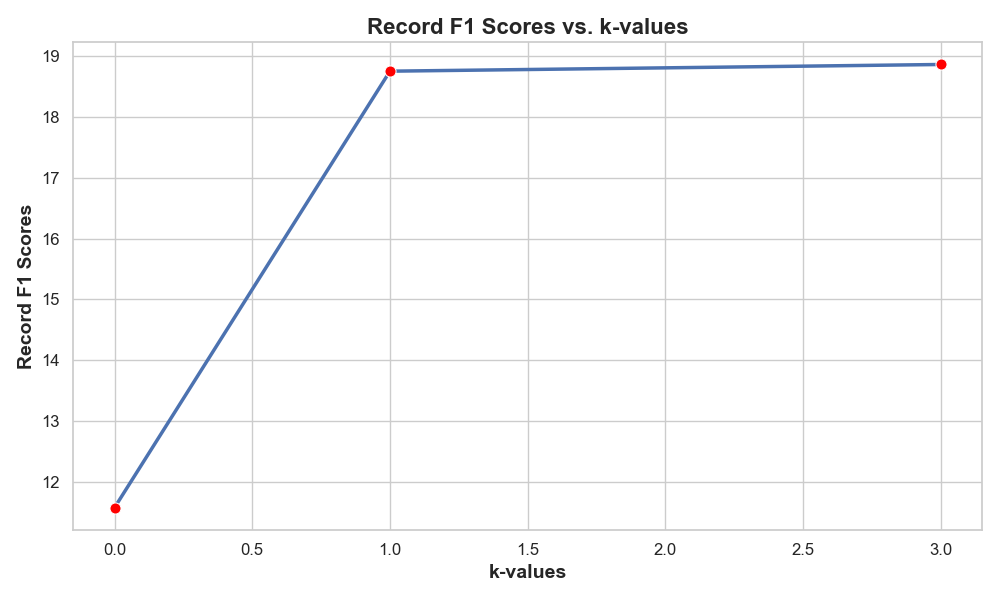
\includegraphics[width=0.8\textwidth]{Figure_1.png}
    \caption{F1 Scores vs. k-values}
    \label{fig:Figure_1}
\end{figure}

\newpage

\paragraph{Qualitative Error Analysis:} Conduct a detailed error analysis for each of the three models. Identify common error types and discuss possible reasons for these errors in \autoref{tab:qualitative}.

You must identify at least three classes of errors for the queries, and use examples to illustrate them.
It must be clear what model makes the errors you are analyzing. 
If you identified the same type of error for different models, you don't need to duplicate the descriptions, but you need to clearly specify an example for each of the model, indicate the statistics for each model, and specify to which model each statistics correspond to.
You may add more rows to the table.


\begin{landscape}
\begin{table}
  \centering
  \begin{tabular}{p{2cm}p{2cm}p{10cm}p{6cm}p{2cm}}
    \toprule
    \textbf{Error Type} & \textbf{Relevant Models} & \textbf{Example of Error (All from T5 FT)} & \textbf{Error Description} & \textbf{Statistics} \\
    \midrule
    \textcolor{gray}{Unnecessary Conditions} & \textcolor{gray}{T5 fine-tuned} & \textcolor{gray}{INCORRECT:\newline SELECT DISTINCT flight\_1.flight\_id FROM flight flight\_1, airport airport\_1, airport\_service airport\_service\_1, city city\_1 WHERE flight\_1.to\_airport = airport\_1.airport\_code AND airport\_1.airport\_code = 'MKE' AND flight\_1.from\_airport = airport\_service\_1.airport\_code AND airport\_service\_1.city\_code = city\_1.city\_code AND 1 = 1} & \textcolor{gray}{Unnecessary tautologies such as "AND 1 = 1" that do not contribute to query logic} & \textcolor{gray}{29/466} \\
    \midrule
    \textcolor{gray}{Syntax Issues (Parentheses, Commas, etc.)} & \textcolor{gray}{T5 fine-tuned} & \textcolor{gray}{CORRECT:\newline SELECT DISTINCT aircraft\_1.aircraft\_code FROM aircraft aircraft\_1 WHERE aircraft\_1.aircraft\_code = '734' \newline \newline INCORRECT:\newline SELECT DISTINCT flight\_1.flight\_id FROM flight flight\_1, airport\_service airport\_service\_1, city city\_1 WHERE flight\_1.airline\_code = '734' AND( flight\_1.to\_airport = airport\_service\_1.airport\_code AND airport\_service\_1.city\_code = city\_1.city\_code AND city\_1.city\_name = '734'} & \textcolor{gray}{Unbalanced parentheses or missing commas and other syntax errors} & \textcolor{gray}{131/466} \\
    \midrule
    \textcolor{gray}{Redundant Joins} & \textcolor{gray}{T5 fine-tuned} & \textcolor{gray}{INCORRECT:\newline SELECT DISTINCT flight\_1.flight\_id FROM flight flight\_1, airport\_service airport\_service\_1, city city\_1, airport\_service airport\_service\_2, city city\_2, days days\_1, date\_day date\_day\_1 WHERE flight\_1.from\_airport = airport\_service\_1.airport\_code AND airport\_service\_1.city\_code = city\_1.city\_code AND city\_1.city\_name = 'DENVER' AND( flight\_1.to\_airport = airport\_service\_2.airport\_code AND airport\_service\_2.city\_code = city\_2.city\_code AND city\_2.city\_name = 'BOSTON' AND flight\_1.flight\_days = days\_1.days\_code AND days\_1.day\_name = date\_day\_1.day\_name AND date\_day\_1.year = 1991 AND date\_day\_1.month\_number = 8 AND date\_day\_1.day\_number = 9 )} & \textcolor{gray}{Includes unnecessary joins that do not change the result of the query} & \textcolor{gray}{42/466} \\
    \midrule
    \textcolor{gray}{Incorrect or Mismatched Conditions} & \textcolor{gray}{T5 fine-tuned} & \textcolor{gray}{CORRECT:\newline SELECT DISTINCT aircraft\_1.aircraft\_code FROM aircraft aircraft\_1 WHERE aircraft\_1.basic\_type = 'F28' \newline \newline INCORRECT:\newline SELECT DISTINCT capacity\_1.flight\_id FROM capacity\_1, 'F28'} & \textcolor{gray}{Differences in condition clauses, such as time ranges, city names, or flight\_id references} & \textcolor{gray}{460/466} \\
    \bottomrule
  \end{tabular}
  \caption{This table presents a qualitative analysis of errors found in queries generated by the T5 fine-tuned model on the development set, covering various error types.}
  \label{tab:qualitative}
\end{table}
\end{landscape}


\end{document}